% =============================================================================
\section{Extended Experimental Results}\label{app:extraexp}
% =============================================================================

This appendix describes additional experiments and analyses beyond the main experimental program.

\subsection{Locus stratification by chromatin state}

Compute ECL distributions stratified by Roadmap Epigenomics chromatin states:
\begin{enumerate}[leftmargin=2em, label=(\roman*)]
\item Active TSS (TssA)
\item Flanking active TSS (TssAFlnk)
\item Strong transcription (Tx, TxWk)
\item Active enhancers (Enh, EnhG)
\item Bivalent/poised TSS (TssBiv)
\item Repressed Polycomb (ReprPC, ReprPCWk)
\item Quiescent (Quies)
\end{enumerate}

Expected: active enhancer loci show the longest ECL; quiescent regions show ECL close to zero (model predictions are insensitive to sequence at these loci).

\subsection{Species transfer}

For models trained on human data (Enformer, Borzoi):
\begin{enumerate}[leftmargin=2em, label=(\roman*)]
\item Compute ECL at orthologous loci in mouse (mm10).
\item Compare human vs.\ mouse ECL at matched loci.
\item Expected: ECL may be shorter in mouse if the model has not learned mouse-specific regulatory grammar, despite conserved gene structure.
\end{enumerate}

\subsection{Sequence shuffling controls}

To distinguish compositional effects from syntactic (motif-level) effects:
\begin{enumerate}[leftmargin=2em, label=(\roman*)]
\item Compute ECL on natural sequences (standard protocol).
\item Compute ECL on globally dinucleotide-shuffled sequences (preserving composition but destroying motifs).
\item The difference reveals whether distal ECL reflects motif syntax or base composition.
\end{enumerate}

\subsection{Attention diagnostics for transformer models}

For Enformer and Borzoi:
\begin{enumerate}[leftmargin=2em, label=(\roman*)]
\item Extract attention maps $A^{(l)}_{r,i}$ from each layer $l$ and head.
\item Compute attention-based ``context profile'': $a(d) = \frac{1}{H}\sum_h \frac{1}{|L|}\sum_l A^{(l,h)}_{r,i}$ averaged over heads and layers.
\item Correlate attention profile decay with perturbation influence profile decay.
\item Expected: moderate but imperfect correlation. Attention weight $\neq$ functional influence~\citep{Kendiukhov2026MechInterp}.
\end{enumerate}

\subsection{Context Decay Spectroscopy analysis}

Fit the CDS model (\cref{def:cds}) with $K \in \{1,2,3,4\}$ components to each model's influence profile. Report:
\begin{enumerate}[leftmargin=2em, label=(\roman*)]
\item Optimal $K$ by BIC.
\item Decay rates $\lambda_1 < \lambda_2 < \dots$ and amplitudes $a_k$.
\item Interpretation: $\lambda_1$ (slowest decay) determines long-range ECL; $a_1/\sum a_k$ measures the fraction of influence from long-range processing.
\end{enumerate}
The mixture-of-exponentials model with non-negative amplitudes is non-identifiable when decay rates are close, since $a_k e^{-\lambda_k d} + a_{k+1} e^{-\lambda_{k+1} d} \approx (a_k + a_{k+1}) e^{-\lambda_k d}$ in that regime. We recommend enforcing identifiability by a minimum-separation constraint $\lambda_{k+1}/\lambda_k \ge \rho$ for some $\rho > 1$ (e.g., $\rho = 2$), reported alongside the fitted parameters.

\begin{figure}[t]
\centering
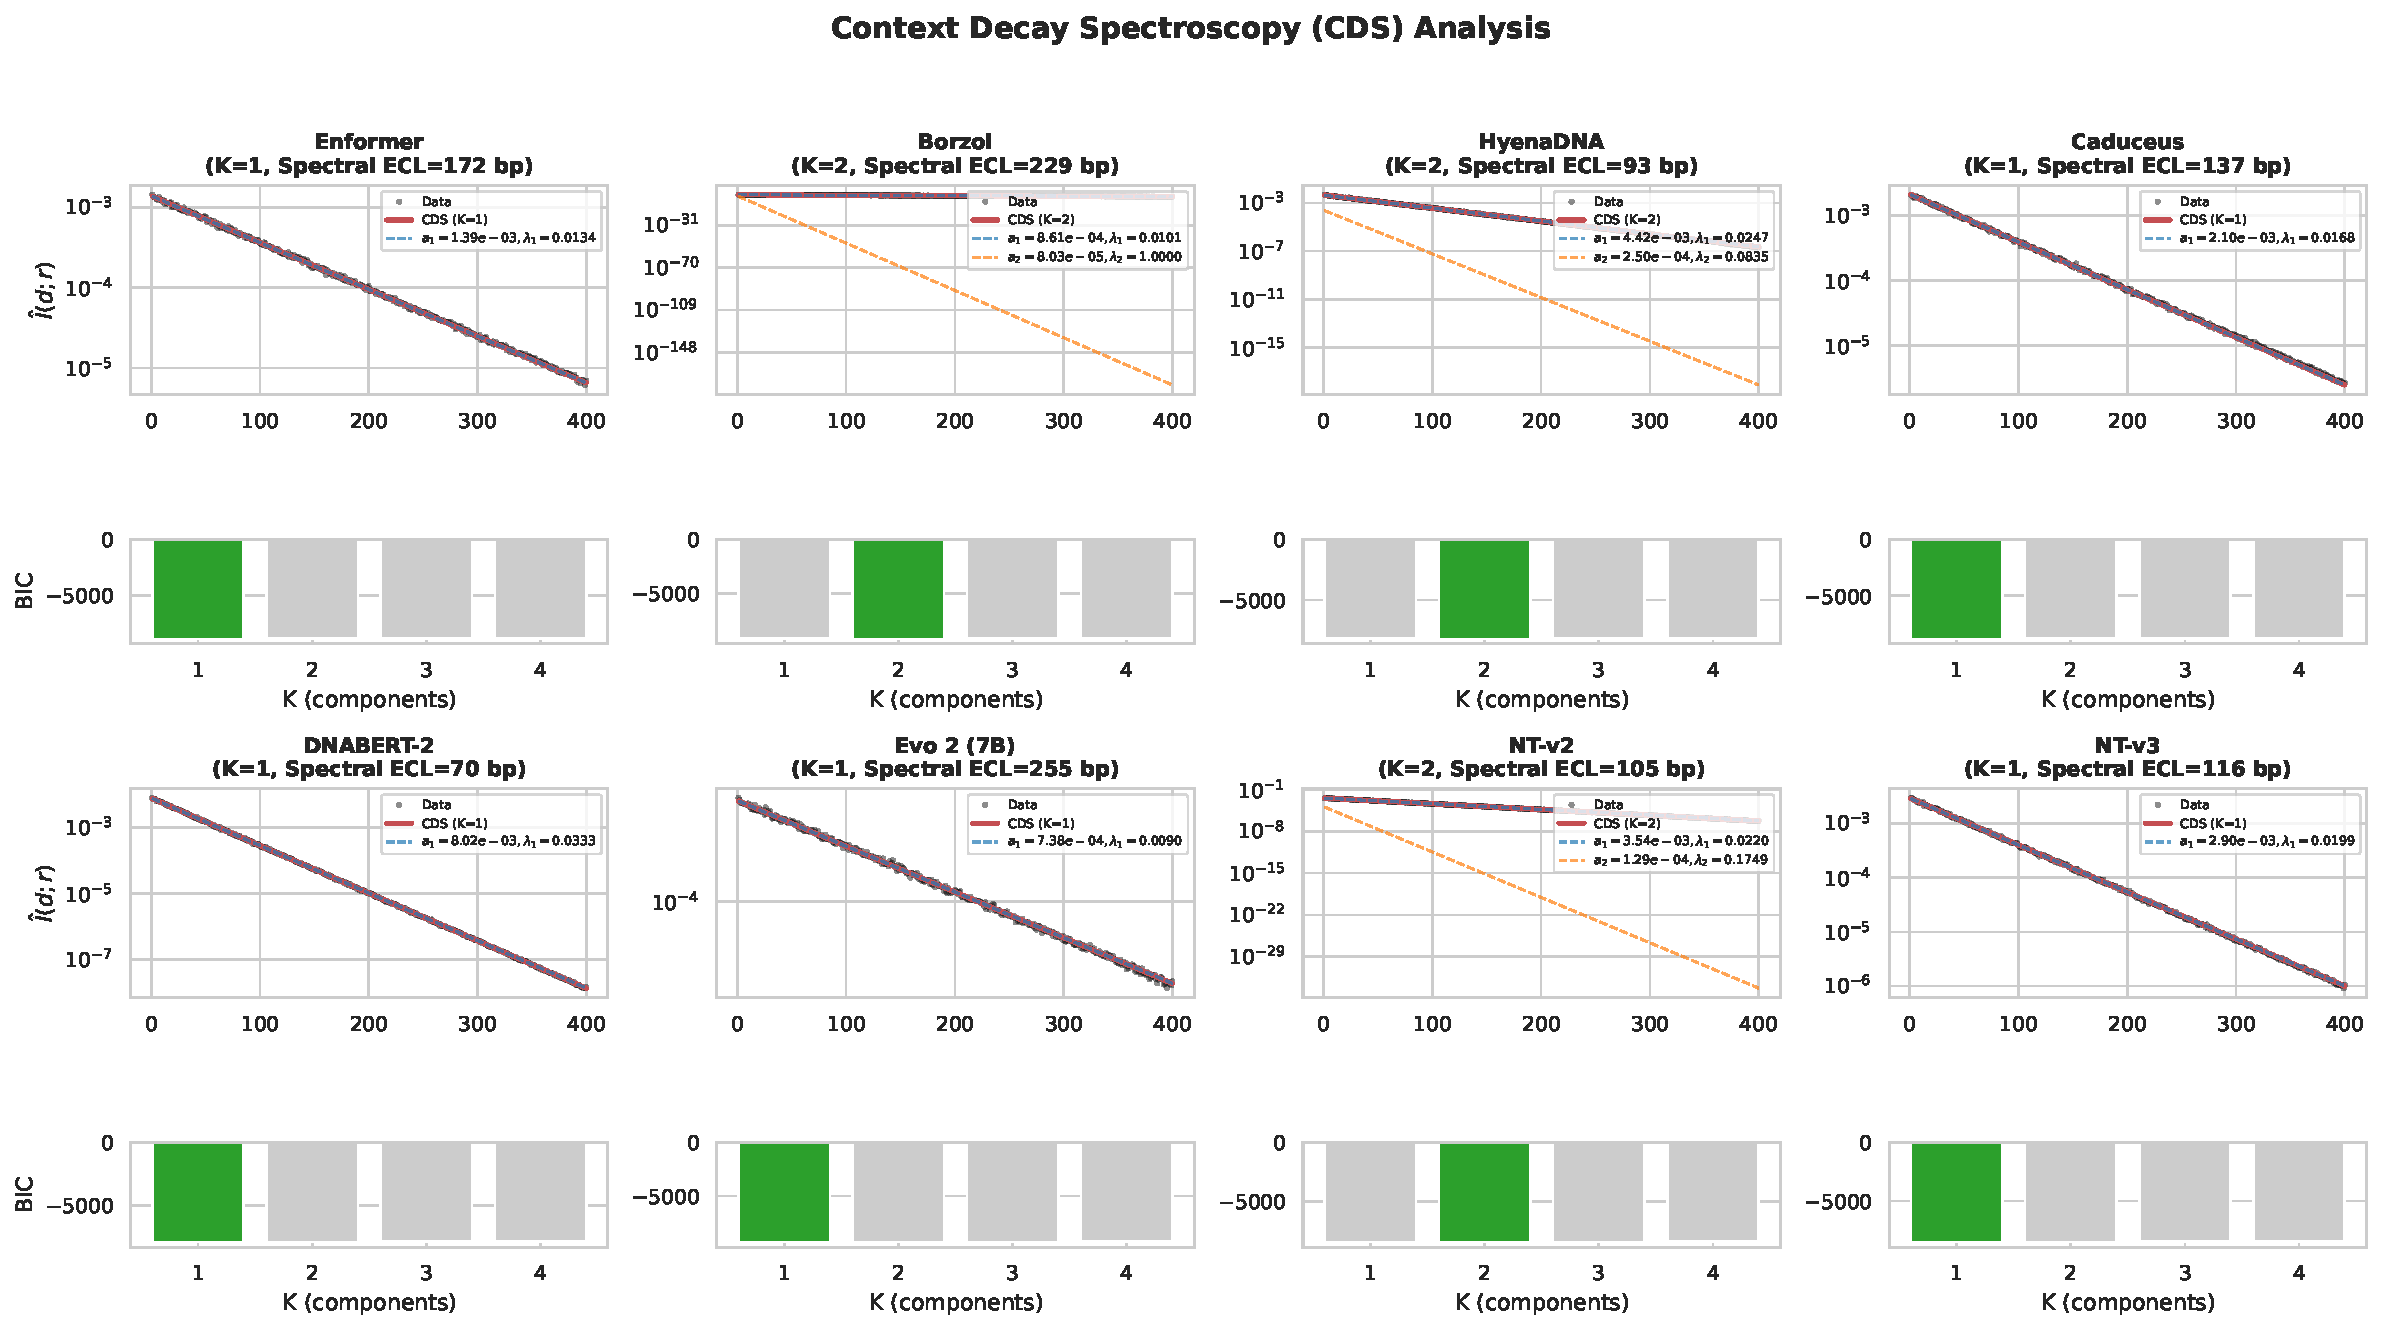
\includegraphics[width=\textwidth]{figures/figA1_cds_analysis.pdf}
\caption{Context Decay Spectroscopy (CDS) analysis for eight models (synthetic surrogates). Top panels: log-scale influence profiles (black dots) with CDS fits (red lines) and individual exponential components (dashed). Bottom panels: BIC model selection over $K \in \{1,2,3,4\}$ components (green = selected). Models with longer decay lengths require fewer components; short-context models exhibit multi-scale decay structure.}
\label{fig:cds_analysis}
\end{figure}

\subsection{ECL vs.\ model performance}

Correlate ECL$_{0.9}$ with downstream task performance (Pearson $r$) across models:
\begin{enumerate}[leftmargin=2em, label=(\roman*)]
\item Gene expression prediction (MSE on held-out genes).
\item Variant effect prediction (Spearman $\rho$ with GTEx eQTL effect sizes).
\item Chromatin accessibility prediction (AUROC on ENCODE peaks).
\end{enumerate}

Expected: models with larger ECL at relevant loci achieve better long-range prediction, but the correlation may be weak if local motif features dominate performance.

\subsection{ECD analysis}

Report Effective Context Dimension distributions across models and locus classes. ECD reveals whether a model distributes influence broadly (high ECD, genuinely using many positions) or concentrates on a few key positions (low ECD).

\begin{figure}[t]
\centering
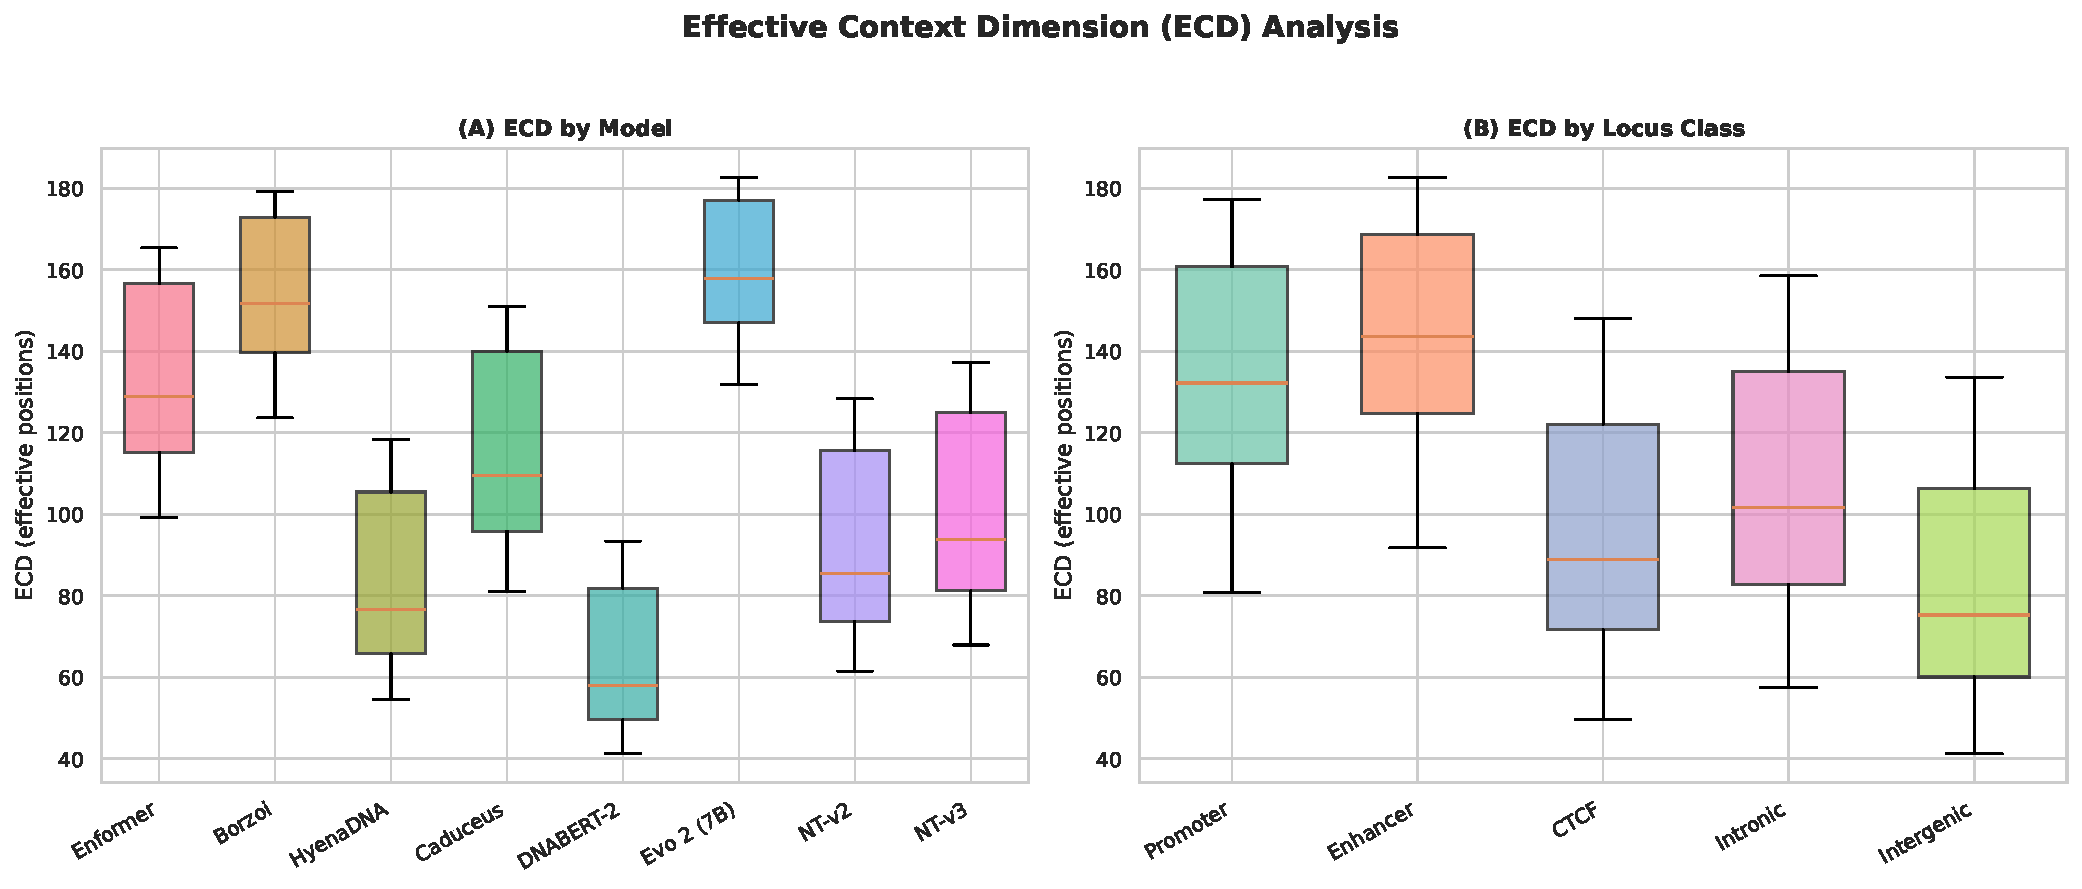
\includegraphics[width=\textwidth]{figures/figA2_ecd_analysis.pdf}
\caption{Effective Context Dimension (ECD) distributions. (A)~ECD by model, aggregated across locus classes. Longer-context models (Evo~2, Borzoi) exhibit higher ECD. (B)~ECD by locus class, aggregated across models. Enhancer and promoter loci show higher ECD than intergenic regions, consistent with their richer regulatory context.}
\label{fig:ecd_analysis}
\end{figure}

\subsection{Positional bias analysis}

Test for ``lost in the middle'' effects in genomic models:
\begin{enumerate}[leftmargin=2em, label=(\roman*)]
\item For Enformer (196~kb window), compute $\cI(i;r)$ for reference positions $r$ at the center, 25\% from edge, and near the edge.
\item Plot influence as a function of absolute position (not distance from $r$).
\item Expected: if positional encoding creates edge bias, influence will be higher for absolute positions near the boundaries regardless of $r$.
\end{enumerate}
